% replace all text with your own text.
% in this template few examples are mention
\chapter{Methodology}
\label{ch:method} % Label for method chapter


\section{Dataset Description}

The Kaggle heart disease dataset\cite{lapp-heart-disease-dataset-1988}, which has 1025 samples with 14 attributes each, was used in this investigation. The dataset includes a number of clinical characteristics that are frequently used to determine whether a patient has cardiac disease. Each sample has the following characteristics and represents a patient:

\begin{enumerate}
    \item Age (\textit{age}): The age of the patient in years.
    \item Sex (\textit{sex}): The gender of the patient (1 = male, 0 = female).
    \item Chest Pain Type (\textit{cp}): The type of chest pain experienced by the patient, categorized into four types: typical angina (1), atypical angina (2), non-anginal pain (3), and asymptomatic (4).
    \item Resting Blood Pressure (\textit{trestbps}): The resting blood pressure of the patient in mm Hg.
    \item Serum Cholesterol (\textit{chol}): The serum cholesterol level of the patient in mg/dl.
    \item Fasting Blood Sugar (\textit{fbs}): The fasting blood sugar level of the patient, where 1 indicates a fasting blood sugar level greater than 120 mg/dl and 0 indicates a level less than or equal to 120 mg/dl.
    \item Resting Electrocardiographic Results (\textit{restecg}): The resting electrocardiographic results of the patient, categorized into three types: normal (0), having ST-T wave abnormality (1), and showing probable or definite left ventricular hypertrophy (2).
    \item Maximum Heart Rate Achieved (\textit{thalach}): The maximum heart rate achieved by the patient.
    \item Exercise-Induced Angina (\textit{exang}): Whether the patient experienced exercise-induced angina (1 = yes, 0 = no).
    \item ST Depression Induced by Exercise Relative to Rest (\textit{oldpeak}): The ST depression induced by exercise relative to rest.
    \item Slope of the Peak Exercise ST Segment (\textit{slope}): The slope of the peak exercise ST segment, categorized into three types: upsloping (1), flat (2), and downsloping (3).
    \item Number of Major Vessels Colored by Fluoroscopy (\textit{ca}): The number of major vessels colored by fluoroscopy, ranging from 0 to 3.
    \item Thalassemia (\textit{thal}): The thalassemia status of the patient, categorized into three types: normal (3), fixed defect (6), and reversible defect (7).
    \item Target (\textit{target}): The presence of heart disease in the patient, where 1 indicates the presence of heart disease and 0 indicates the absence of heart disease.
\end{enumerate}
\subsection{Target Variable}
The target variable, \textit{target}, indicates the presence of heart disease and is binary, where 1 represents disease present and 0 represents disease not present.

\subsection{Data Types}
The dataset consists of the following features with their respective data types:
\begin{itemize}
    \item \textbf{age}: integer
    \item \textbf{sex}: integer
    \item \textbf{cp}: integer
    \item \textbf{trestbps}: integer
    \item \textbf{chol}: integer
    \item \textbf{fbs}: integer
    \item \textbf{restecg}: integer
    \item \textbf{thalach}: integer
    \item \textbf{exang}: integer
    \item \textbf{oldpeak}: float
    \item \textbf{slope}: integer
    \item \textbf{ca}: integer
    \item \textbf{thal}: integer
    \item \textbf{target}: integer
\end{itemize}




\begin{figure}
    \centering
    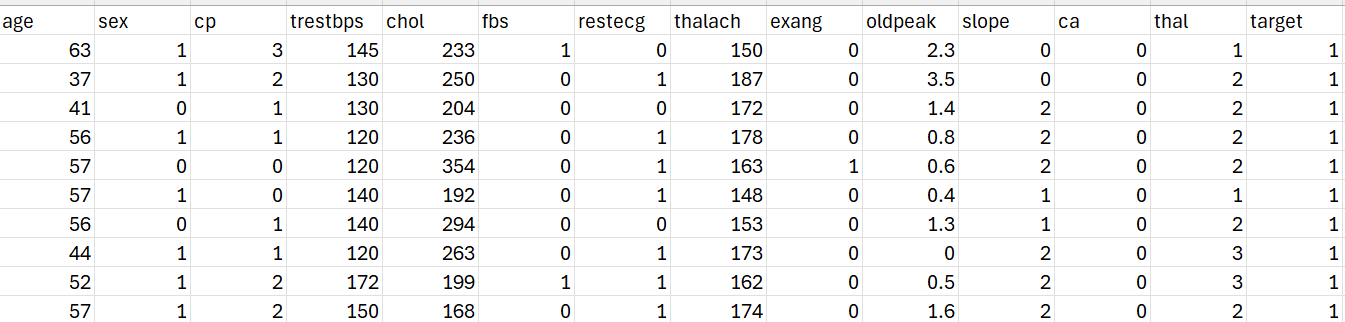
\includegraphics[width=1.0\textwidth]{figures/Datasettop10patients.png}
    \caption{Top 10 patient data from dataset}
    \label{fig:example}
\end{figure}
\section{Software Used}
The implementation and comparison of SVM and Random Forest models were performed using Python along with the following libraries:
\begin{itemize}
    \item \textbf{Python}: Python programming language was used as the primary language for coding the models.
    \item \textbf{pandas}: The pandas library was utilized for data manipulation and analysis, including reading the dataset, creating dataframes, and structuring the data.
    \item \textbf{scikit-learn (sklearn)}: The scikit-learn library was used for implementing the SVM and Random Forest algorithms, as well as for data preprocessing, model training, and evaluation.
\end{itemize}
These libraries provided the necessary tools and functions to effectively implement and compare the models, ensuring a robust and efficient analysis of the dataset.

\section{Data preparation and cleaning}
As an initial step for preparing and cleaning data in this study, a dataset comprising 1025 samples is read from a CSV file and transformed into a table using Python's pandas library. This procedure involves loading the dataset, associating the columns with their corresponding values, and constructing a table containing the samples. This process is crucial for structuring the data in an organized manner, which will simplify subsequent tasks such as data cleaning, managing missing values, and preparing the data for training and testing the SVM and Random Forest models.
\subsection{Dataset Loading and Data Type Definition}To prepare the data for analysis, I first categorized each column based on its data type. Subsequently, I imported the dataset from a CSV file into a Pandas DataFrame. This step was crucial for organizing and analyzing the data efficiently.
\begin{figure}
    \centering
    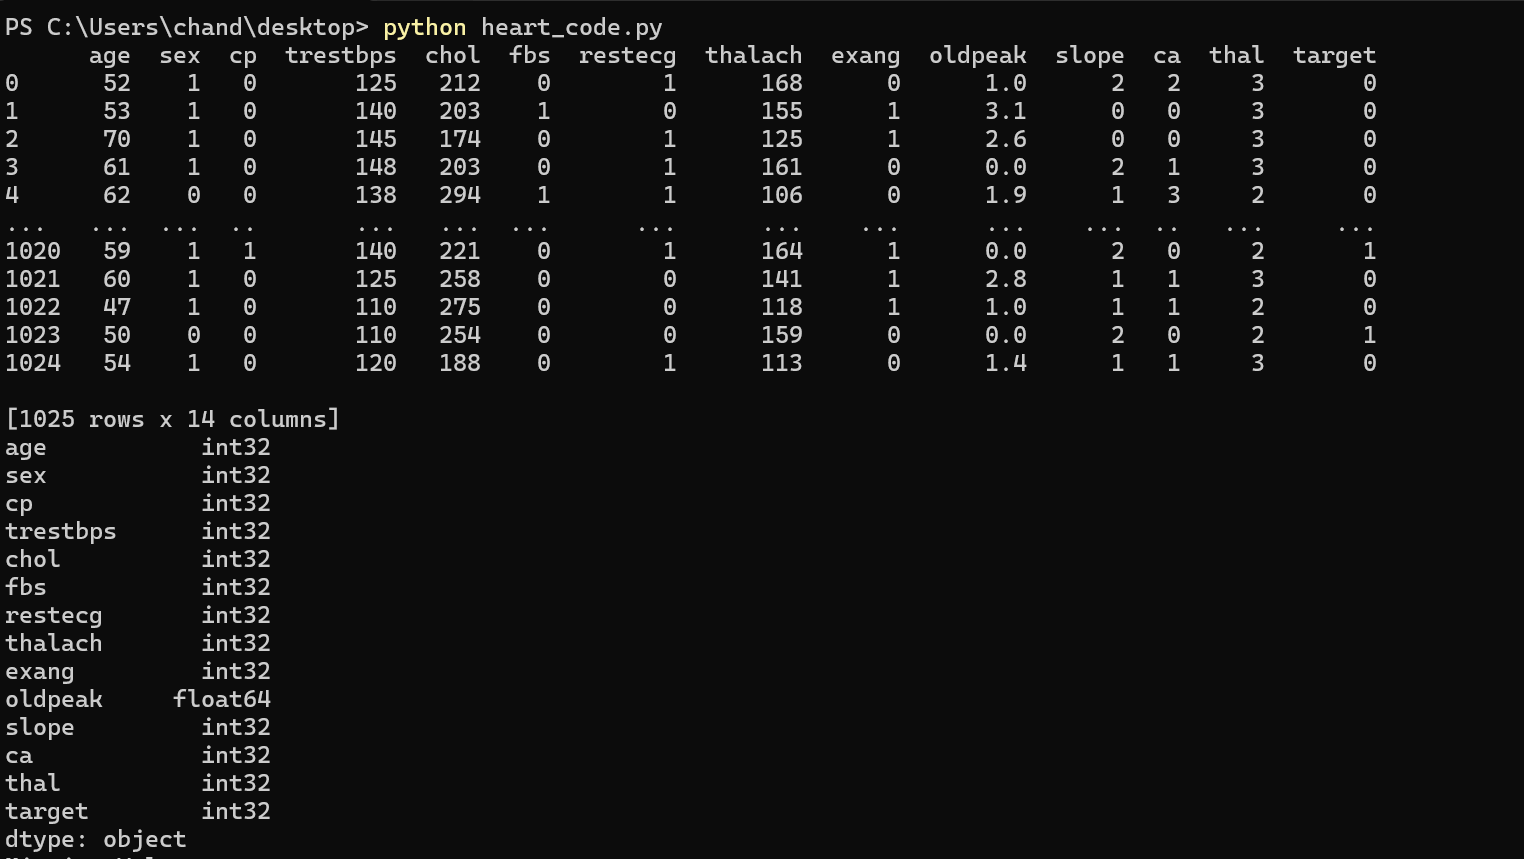
\includegraphics[width=1.0\textwidth]{figures/loaddata.png}
    \caption{Load data and data type definition}
    \label{fig:example}
\end{figure}
Table~\ref{tab:algo_temp} may suit you the best. 
\begin{table}[ht!]
    \centering
    \caption{Example of an algorithm analysis type report structure}
    \label{tab:algo_temp}
    \begin{tabular}{lll}     
        \toprule                   
        Chapter 1 & Introduction  &    \\        
        Chapter 2 & Literature Review  &    \\                
        Chapter 3 & Methodology   &    \\
        &               & Algorithms descriptions  \\
        &               & Implementations   \\
        &               & Experiments design   \\
        Chapter 4 & Results       &  \\
        Chapter 5 & Discussion and Analysis  &    \\
        Chapter 6 & Conclusion and Future Work  &    \\        
        Chapter 7 & Reflection  &    \\          
        \bottomrule
    \end{tabular}
\end{table}


\subsection{Example of a science lab-type main text structure}
If you are doing a science lab experiment type of project, you may use the  methodology section suggested in Table~\ref{tab:lab_temp}. In this kind of project, you may refer to the ``Methodology'' section as ``Materials and Methods.''
\begin{table}[ht!]
    \centering
    \caption{Example of a science lab experiment-type report structure}
    \label{tab:lab_temp}
    \begin{tabular}{lll}     
        \toprule                   
        Chapter 1 & Introduction  &    \\        
        Chapter 2 & Literature Review  &    \\                
        Chapter 3 & Materials and Methods   &    \\
        &               & Problems (tasks) description  \\
        &               & Materials \\        
        &               & Procedures  \\                
        &               & Implementations   \\
        &               & Experiment set-up   \\
        Chapter 4 & Results       &  \\
        Chapter 5 & Discussion and Analysis  &    \\
        Chapter 6 & Conclusion and Future Work  &    \\        
        Chapter 7 & Reflection  &    \\          
        \bottomrule
    \end{tabular}
\end{table}

\section{Example of an Equation in \LaTeX}
Eq.~\ref{eq:eq_example} [note that this is an example of an equation's in-text citation] is an example of an equation in \LaTeX. In Eq.~\eqref{eq:eq_example}, $ s $ is the mean of elements $ x_i \in \mathbf{x} $: 

\begin{equation}
\label{eq:eq_example} % label used to refer the eq in text
s = \frac{1}{N} \sum_{i = 1}^{N} x_i. 
\end{equation}

Have you noticed that all the variables of the equation are defined using the \textbf{in-text} maths command \$.\$, and Eq.~\eqref{eq:eq_example} is treated as a part of the sentence with proper punctuation? Always treat an equation or expression as a part of the sentence. 

\section{Example of a Figure in \LaTeX}
Figure~\ref{fig:chart_a} is an example of a figure in \LaTeX. For more details, check the link:

\href{https://en.wikibooks.org/wiki/LaTeX/Floats,_Figures_and_Captions}{wikibooks.org/wiki/LaTeX/Floats,\_Figures\_and\_Captions}.

\noindent
Keep your artwork (graphics, figures, illustrations) clean and readable. At least 300dpi is a good resolution of a PNG format artwork. However, an SVG format artwork saved as a PDF will produce the best quality graphics. There are numerous tools out there that can produce vector graphics and let you save that as an SVG file and/or as a PDF file. One example of such a tool is the ``Flow algorithm software''. Here is the link for that: \href{http://www.flowgorithm.org/download/}{flowgorithm.org}.
\begin{figure}[ht]
    \centering
    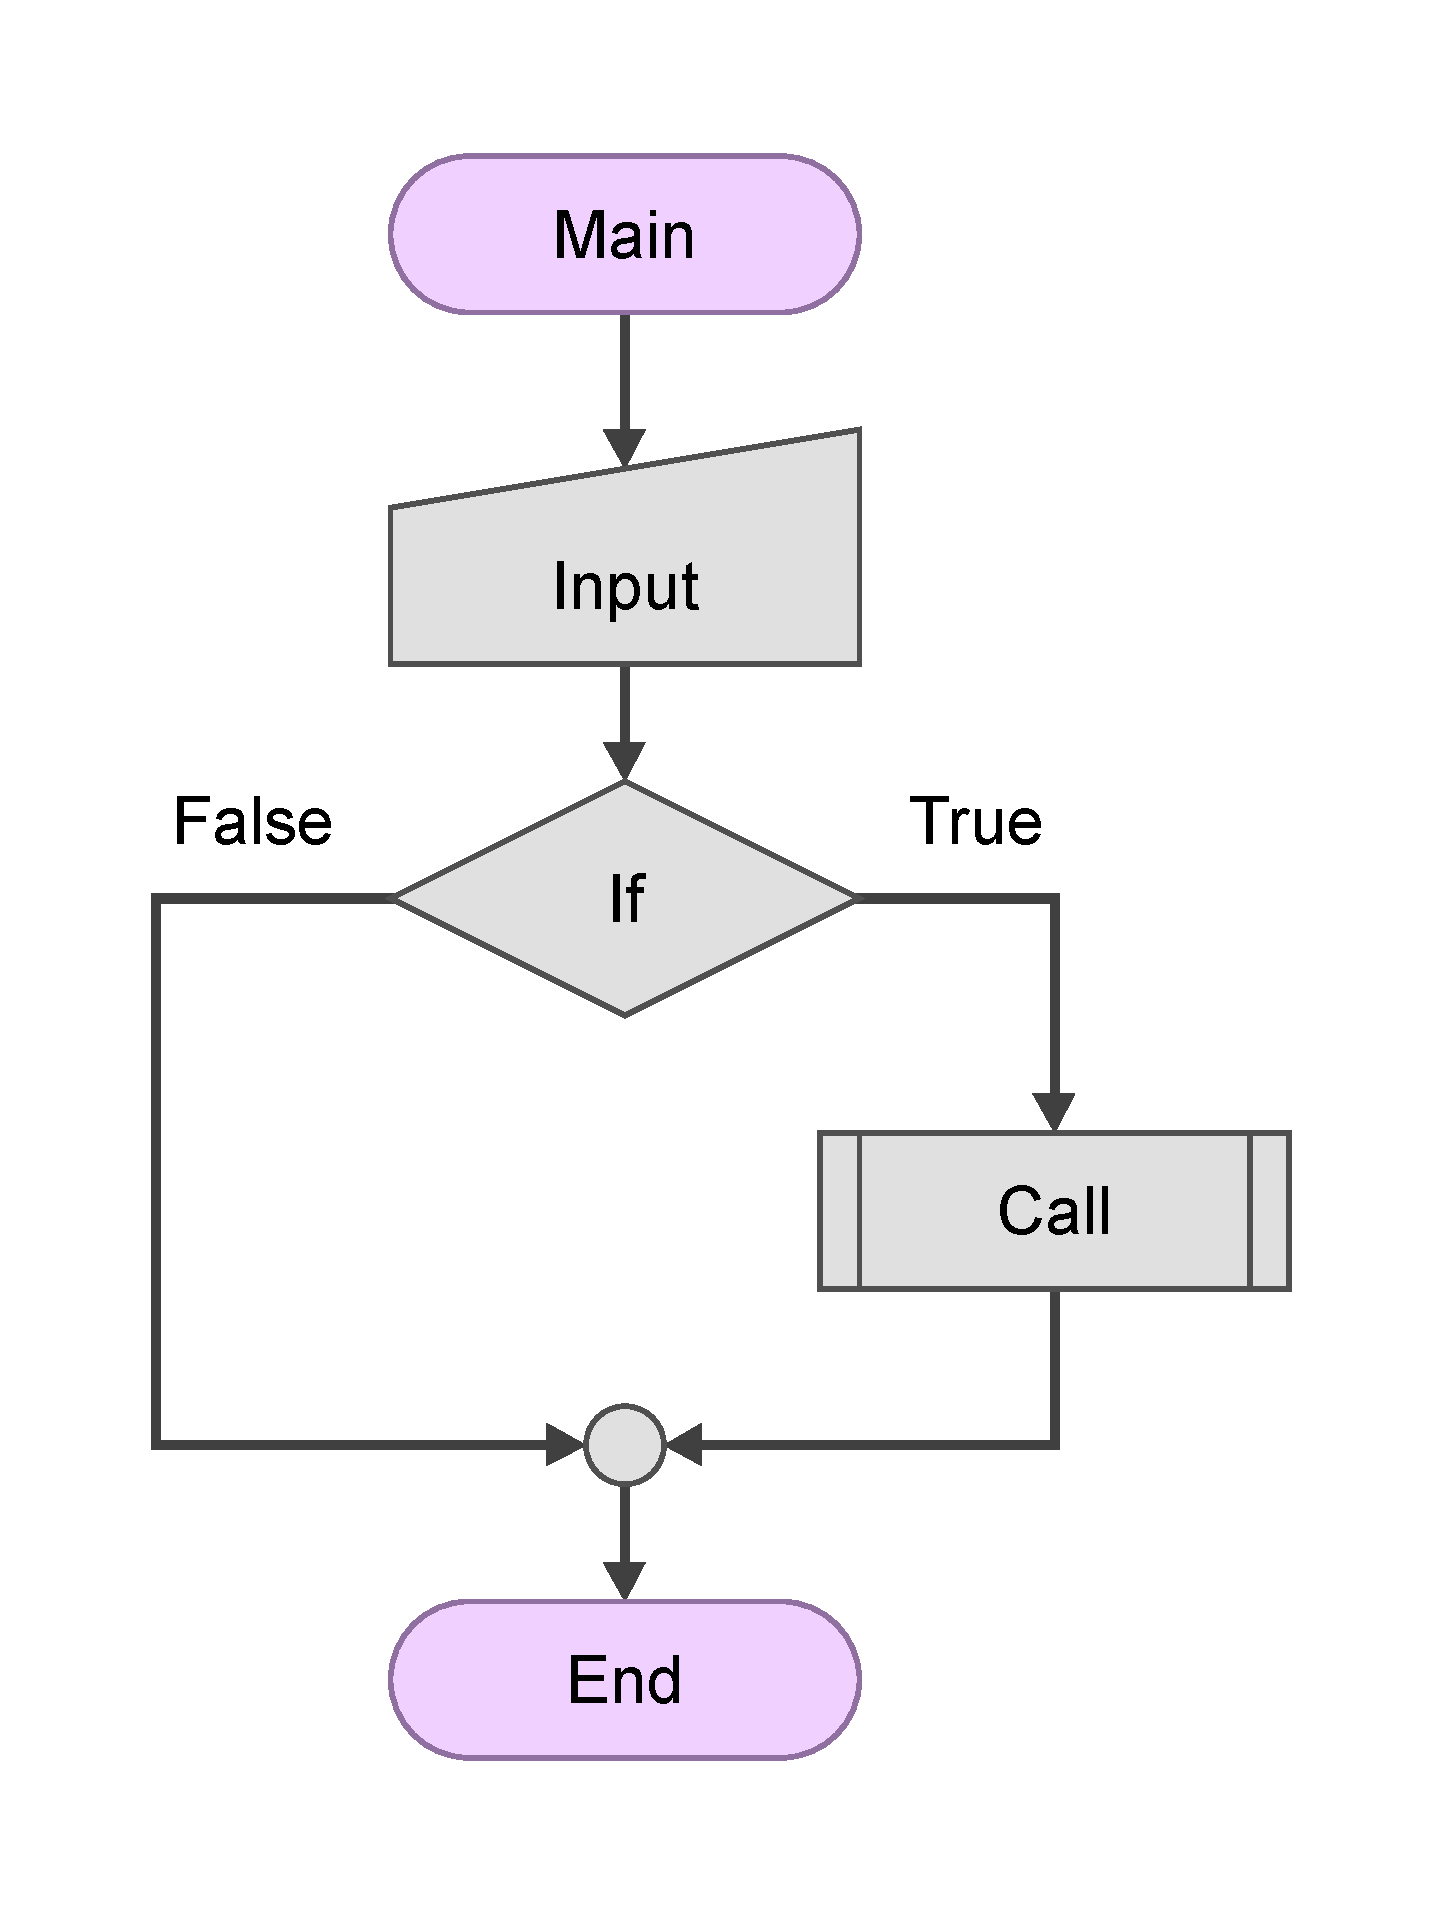
\includegraphics[scale=0.3]{figures/chart.pdf}
    \caption{Example figure in \LaTeX.}
    \label{fig:chart_a}
\end{figure}

\clearpage %  use command \clearpage when you want section or text to appear in the next page.

\section{Example of an algorithm in \LaTeX}
Algorithm~\ref{algo:algo_example} is a good example of an algorithm in \LaTeX.  
\begin{algorithm}
    \caption{Example caption: sum of all even numbers}
    \label{algo:algo_example}
    \begin{algorithmic}[1]
        \Require{$ \mathbf{x}  = x_1, x_2, \ldots, x_N$}
        \Ensure{$EvenSum$ (Sum of even numbers in $ \mathbf{x} $)}
        \Statex
        \Function{EvenSummation}{$\mathbf{x}$}
        \State {$EvenSum$ $\gets$ {$0$}}
        \State {$N$ $\gets$ {$length(\mathbf{x})$}}
        \For{$i \gets 1$ to $N$}                    
        \If{$ x_i\mod 2 == 0$}  \Comment check if a number is even?
        \State {$EvenSum$ $\gets$ {$EvenSum + x_i$}}
        \EndIf
        \EndFor
        \State \Return {$EvenSum$}
        \EndFunction
    \end{algorithmic}
\end{algorithm}
 
\section{Example of code snippet  in \LaTeX}

Code Listing~\ref{list:python_code_ex} is a good example of including a code snippet in a report. While using code snippets, take care of the following:
\begin{itemize}
    \item do not paste your entire code (implementation) or everything you have coded. Add code snippets only. 
    \item The algorithm shown in Algorithm~\ref{algo:algo_example} is usually preferred over code snippets in a technical/scientific report. 
    \item Make sure the entire code snippet or algorithm stays on a single page and does not overflow to another page(s).  
\end{itemize}

Here are three examples of code snippets for three different languages (Python, Java, and CPP) illustrated in Listings~\ref{list:python_code_ex}, \ref{list:java_code_ex}, and \ref{list:cpp_code_ex} respectively.  

\begin{lstlisting}[language=Python, caption={Code snippet in \LaTeX ~and  this is a Python code example}, label=list:python_code_ex]
import numpy as np

x  = [0, 1, 2, 3, 4, 5] # assign values to an array
evenSum = evenSummation(x) # call a function

def evenSummation(x):
    evenSum = 0
    n = len(x)
    for i in range(n):
        if np.mod(x[i],2) == 0: # check if a number is even?
            evenSum = evenSum + x[i]
    return evenSum
\end{lstlisting}

Here we used  the ``\textbackslash clearpage'' command and forced-out the second listing example onto the next page. 
\clearpage  %
\begin{lstlisting}[language=Java, caption={Code snippet in \LaTeX ~and  this is a Java code example}, label=list:java_code_ex]
public class EvenSum{ 
    public static int evenSummation(int[] x){
        int evenSum = 0;
        int n = x.length;
        for(int i = 0; i < n; i++){
            if(x[i]%2 == 0){ // check if a number is even?
                evenSum = evenSum + x[i];
            }
        }
        return evenSum;     
    }
    public static void main(String[] args){ 
        int[] x  = {0, 1, 2, 3, 4, 5}; // assign values to an array
        int evenSum = evenSummation(x);
        System.out.println(evenSum);
    } 
} 
\end{lstlisting}


\begin{lstlisting}[language=C, caption={Code snippet in \LaTeX ~and  this is a C/C++ code example}, label=list:cpp_code_ex]
int evenSummation(int x[]){
    int evenSum = 0;
    int n = sizeof(x);
    for(int i = 0; i < n; i++){
        if(x[i]%2 == 0){ // check if a number is even?
            evenSum = evenSum + x[i];
    	}
    }
    return evenSum;     
}

int main(){
    int x[]  = {0, 1, 2, 3, 4, 5}; // assign values to an array
    int evenSum = evenSummation(x);
    cout<<evenSum;
    return 0;
}
\end{lstlisting}



\section{Example of in-text citation style}
\subsection{Example of the equations and illustrations placement and reference in the text}
Make sure whenever you refer to the equations, tables, figures, algorithms,  and listings for the first time, they also appear (placed) somewhere on the same page or in the following page(s). Always make sure to refer to the equations, tables and figures used in the report. Do not leave them without an \textbf{in-text citation}. You can refer to equations, tables and figures more them once.

\subsection{Example of the equations and illustrations style}
Write \textbf{Eq.} with an uppercase ``Eq`` for an equation before using an equation number with (\textbackslash eqref\{.\}). Use ``Table'' to refer to a table, ``Figure'' to refer to a figure, ``Algorithm'' to refer to an algorithm and ``Listing'' to refer to listings (code snippets). Note that, we do not use the articles ``a,'' ``an,'' and ``the'' before the words Eq., Figure, Table, and Listing, but you may use an article for referring the words figure, table, etc. in general.

For example, the sentence ``A report structure is shown in \textbf{the} Table~\ref{tab:gen_template}'' should be written as ``A report structure is shown \textbf{in} Table~\ref{tab:gen_template}.'' 
 

\section{Summary}
Write a summary of this chapter.

~\\[5em]
\noindent
{\huge\textbf{Note:}} In the case of \textbf{software engineering} project a Chapter ``\textbf{Testing and Validation}'' should precede the ``Results'' chapter. See Section~\ref{subsec:se_chpters} for report organization of such project. 

